\documentclass{lkx_paper}

\title{Cosmological Constraints from \\Baryonic Acoustic Oscillations}
\date{April 2025}
\author{Lev Kruglyak}

\lkxbib{final-paper}

\usepackage{graphicx}
\usepackage{float}
\usepackage[skip=2pt]{caption}
\usepackage{titling}
\setlength{\droptitle}{-5em} 

\renewcommand{\d}{{\mathrm{d}}}
\renewcommand{\b}{{\mathrm{b}}}
\renewcommand{\c}{{\mathrm{c}}}
\newcommand{\bc}{{\mathrm{bc}}}
\newcommand{\K}{{\mathrm{K}}}
\newcommand{\m}{{\mathrm{m}}}
\newcommand{\DE}{{\mathrm{DE}}}
\newcommand{\MC}{{\mathrm{MC}}}
\newcommand{\eff}{{\mathrm{eff}}}
\newcommand{\CMB}{\mathrm{CMB}}

\newcommand{\LCDM}{$\Lambda\mathrm{CDM}$~}
\newcommand{\wwCDM}{{$w_0 w_a\mathrm{CDM}$~}}

\DeclareMathOperator{\diag}{{\operatorname{diag}}}

\newcommand{\MM}{{\mathcal{M}}}
\newcommand{\DD}{{\mathcal{D}}}
\newcommand{\UU}{{\mathcal{U}}}
\newcommand{\NN}{{\mathcal{N}}}
\newcommand{\LL}{{\mathcal{L}}}
\usepackage{bm}
\newcommand{\pms}{{\bm{\theta}}}
\newcommand{\Neff}{{N_\mathrm{eff}}}

\usepackage{siunitx}
\renewcommand{\si}[1]{\qty[per-mode = symbol]{#1}{}}
\providecommand{\Mpcsi}[1]{\qty{#1}{\mathrm{Mpc}}}
\providecommand{\eVsi}[1]{\qty{#1}{\mathrm{eV}}}
\providecommand{\Hsi}[1]{\qty{#1}{\km\,\s^{-1}\,\mathrm{Mpc}^{-1}}}

\begin{document}

In this paper, we use measurements of baryon acoustic oscillation (BAO) measurements by the Dark Energy Spectroscopic Instrument (DESI) to obtain constraints on cosmological parameters in the \LCDM model. This analysis has already been done in \cite{desicollaboration2025desidr2resultsii}, here we attempt to recreate some of the constraints obtained in that paper.

\subsection*{The \LCDM Model}
We begin with a brief review of the \LCDM model. The base geometry is the FLRW metric -- we assume further that it is flat.
Energy density in the model is thus split into five species: baryonic matter $\Omega_\b$, cold (i.e. non-relativistic) dark matter $\Omega_\c$, electromagnetic radiation $\Omega_\gamma$, curvature $\Omega_\K$, neutrinos $\Omega_\nu$, and dark energy $\Omega_\DE$. Note that the curvature energy density $\Omega_K=0$ is trivial, so we do not include it here. Baryonic and cold dark matter are grouped as $\Omega_\bc=\Omega_\b+\Omega_\c$, and non-relativistic matter including neutrinos is grouped as $\Omega_\m=\Omega_\bc+\Omega_\m$.
Using standard equation of state parameters for $\Omega_\bc$, $\Omega_\gamma$, and $\Omega_K$, we can write the time-dependent Hubble parameter as:
\begin{equation}
  \frac{H(z)}{H_0} = 
  \left[\Omega_\bc(1+z)^3 + \Omega_\gamma(1+z)^4+\Omega_\nu\frac{\rho_\nu(z)}{\rho_{\nu,0}} + \Omega_\DE \frac{\rho_\DE(z)}{\rho_{\DE,0}}\right]^{1/2}.
\end{equation}
The energy density of neutrinos begins scaling as $(1+z)^4$ at high redshifts and transitions to $(1+z)^3$. Throughout, we assume the existence of a single species of massive neutrino with mass $m_\nu = \eVsi{0.06}$ and $\Neff=3.044$. In the base \LCDM model, we assume that dark energy is constant over time, namely that $\rho_{\DE}(z)/\rho_{\DE,0}=1$. We remove this assumption later in the paper.

When performing Bayesian analysis on the \LCDM model, we sample along the six independent parameters of the model: $(\omega_\c, \omega_\b, \theta_*, \ln(10^{10}A_s), n_s, \tau)$. The first of these two parameters describe the ratios of cold dark matter and baryonic matter in the universe, i.e. $\omega_\c=\Omega_\c h^2$ and $\omega_\b = \Omega_\b h^2$ where $h=H_0/\Hsi{100}$. The next parameter, $\theta_*$ is the angular size of the sound horizon at the surface of last scattering, i.e.
\begin{equation}
  \theta_* = \frac{r_s(z_*)}{D_A(z_*)}\quad\textrm{where}\quad
  r_s(z) = \int_z^\infty \frac{c_s(z')}{H(z')}\,dz'\quad\textrm{and}\quad D_A(z)=\frac{1}{1+z}\int_0^z\frac{c}{H(z')}\,dz'
\end{equation}
where $z_*\approx 1090$ and $c_s(z)$ is the speed of sound in the primordial photon-baryon fluid. To speed up computation, it is common to approximate $\theta_*$ by a parameter $\theta_\MC$ given by fitting formula in \cite{Lewis_2000}. The remaining parameter $\ln(10^{10} A_s), n_s,$ and $\tau$ are the amplitude and spectral index of the primordial scalar perturbations and the optical depth respectively. 

To perform Bayesian analysis with the CMB and DESI datasets, we use \texttt{Cobaya} \cite{Torrado_2021}, a general purpose Python program for exploring posterior distributions using Monte Carlo samplers. We use \texttt{CAMB} \cite{Lewis:1999bs} as the theoretical model backend for Cobaya analysis and use a Markov Chain Monte Carlo (MCMC) sampler with convergence criterion $R-1<0.01$ in the Gelman-Rubin statistic.

\subsection*{Exploring the CMB $H_0,\Omega_\m$ Degeneracy}

We begin by using the full CMB data from Planck 2018 to derive CMB priors which speed up later computations. We begin with simple uniform priors on the six cosmological parameters, taken from Table 2 of \cite{desicollaboration2024desi2024viicosmological}.We combine this with the full CMB likelihood from Planck 2018, including TT, EE modes for low $\ell$ and NPIPE TTTEEE modes for high $\ell$ as well as PR4 lensing.

\begin{figure}[ht]
  \renewcommand{\arraystretch}{1.2}
  \centering
  \begin{tabular}{|c|c|c|c|c|c|c|}
    \hline
    parameter & $\omega_\c$ & $\omega_b$ & $100\theta_\MC$ & $\ln(10^{10} A_s)$ & $n_s$ & $\tau$\\
    \hline
    default & $\UU[0.001, 0.99]$ & $\UU[0.005, 0.1]$ &$\UU[0.5,10]$ &$\UU[1.61,3.91]$ &$\UU[0.8,1.2]$ & $\UU[0.01, 0.8]$  \\
    \hline
  \end{tabular}
  \medskip
  \caption{Priors for $(\omega_\mathrm{c}, \omega_\mathrm{b}, 100\theta_{\mathrm{MC}}, \ln(10^{10}A_s), n_s, \tau)$.}
\end{figure}

To help calibrate later BAO data, we also add on a BBN consistent prior on $\omega_\b$, namely
\[
    \omega_\b =\Omega_m h^2 \sim \NN(0.02218, 0.00055).
\]
Running \texttt{Cobaya} with these priors, with $\Omega_m$, $H_0$, and $\theta_*$ as derived parameters, we can graph the posterior distribution on $H_0$ and $\Omega_m$. Graphing the direction of $\Omega_\m h^3$, we get a graph of the degeneracy direction of the CMB data. This is a well-known degeneracy, showing that despite the tight bounds which the CMB imposes on many parameters, varied data sources such as BAO are needed to impose constraints on important cosmological parameters.
\begin{figure}[H]
  \centering
  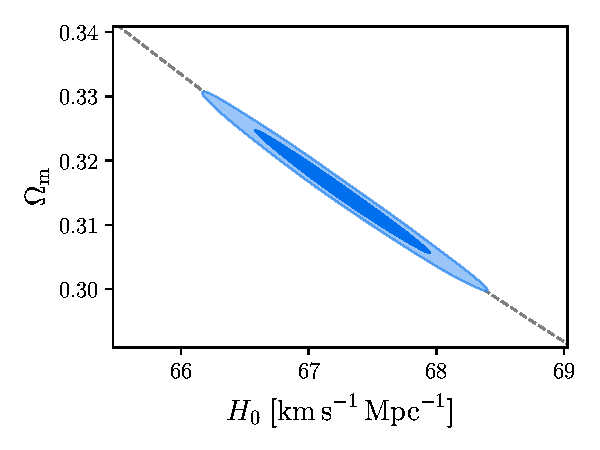
\includegraphics[scale=0.8]{figures/CMB-H0-omegam.pdf}
  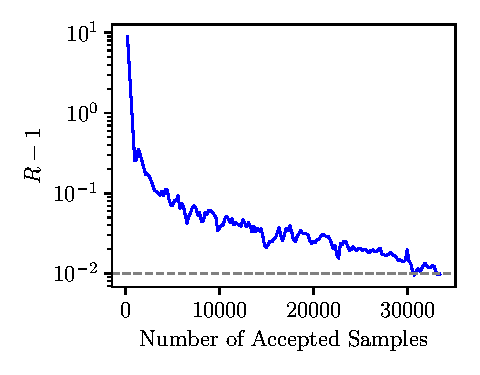
\includegraphics{figures/CMB-R-1.pdf}
  \caption{The $H_0,\Omega_m$ CMB degeneracy. (Planck 2018 + lensing)}
\end{figure}
Using the \texttt{GetDist} python package, we can use the full data of the CMB run to derive the covariance matrix for the parameters $\theta_*, \omega_\b$, and $\omega_\c$. This is useful when we want to approximately include a CMB likelihood without using the entire dataset. Of course, we must be careful to check with the full dataset to ensure the results are within approximation error. 
  \[ 
    \begin{aligned}
      (\theta_*, \omega_\b,&\; \omega_\c) \quad\sim\quad\\ 
                                              &\NN\left(
\begin{bmatrix}
0.01041009 \\
0.02219065 \\
0.11969417
\end{bmatrix},
\begin{bmatrix}
5.10125839\times10^{-12} & 6.40183333\times10^{-11} & -6.09287501\times10^{-10} \\
6.40183333\times10^{-11} & 1.62733275\times10^{-8}  & -6.32279490\times10^{-8}  \\
-6.09287501\times10^{-10} & -6.32279490\times10^{-8} & 1.08987992\times10^{-6}
\end{bmatrix}\right)
    \end{aligned}
\]

\subsection*{Baryonic Acoustic Oscillations}

Baryonic Acoustic Oscillations (BAO) provide a tool to measure the expansion history of the universe by providing a standard ruler given by the characteristic scale which is imprinted on matter clusters in the universe by pre-recombination pressure waves in the primordial baryon-photon fluid.

We now use the DESI DR2 data release, the BBN prior on $\omega_\b$, and a CMB derived prior on $\theta_*$
\[
    100\theta_* \sim \NN(1.04110, 0.00053)
\]
to see what constraints they impose on the $H_0,\Omega_\m$ degeneracy.

\begin{figure}[H]
  \centering
  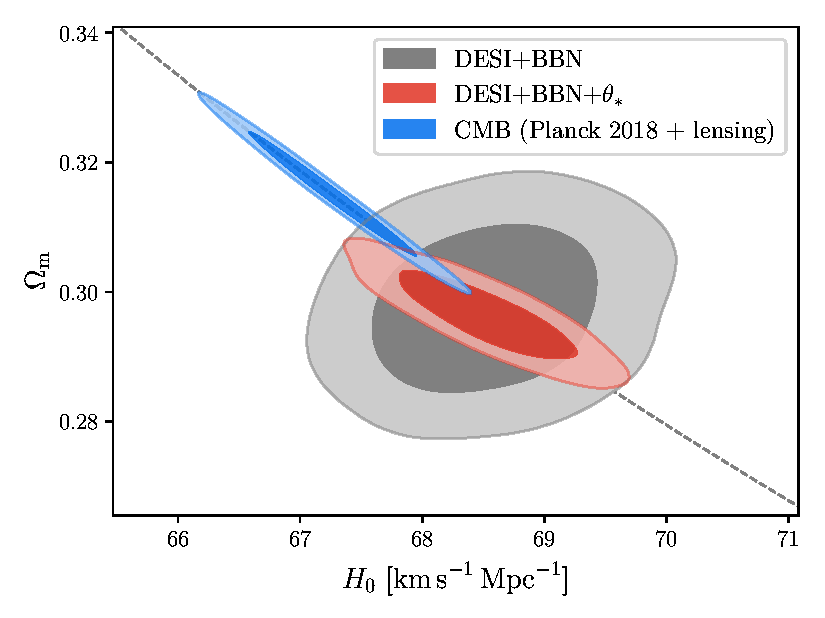
\includegraphics[scale=0.8]{figures/H0-omegam.pdf}
\end{figure}

There is a mild tension ($\approx 2\sigma$) between the DESI+BBN data and the CMB data, but they both generally agree with the $H_0, \Omega_m$ degeneracy of the CMB. Using \texttt{GetDist}, we calculate 68\% limits for $H_0$ and $\Omega_m$, and summarize the bounds in the following table:

\begin{figure}[ht]
  \renewcommand{\arraystretch}{1.2}
  \centering
\begin{tabular}{lcc}
  \hline
  \hline
  &$H_0$ & $\Omega_\m$\\
  \hline
  \textbf{DESI+BBN} & $68.53\pm 0.62$ & $0.2975\pm 0.0085$\\
  \textbf{DESI+BBN+$\theta_*$} & $68.52\pm 0.49$ & $0.2963^{+0.0042}_{-0.0048}$\\
  \hline
  \textbf{CMB} & $67.26\pm 0.46$ & $0.3151\pm 0.0064$\\
  \textbf{DESI+BBN+CMB} & $68.39\pm 0.28$ & $0.2996\pm 0.0035$\\
  \textbf{DESI+BBN+CMB (prior)} & $68.32^{+0.33}_{-0.29}$ & $0.3003^{+0.0037}_{-0.0043}$\\
  \hline
  \hline
\end{tabular}
\medskip
\caption{68\% limits on $H_0$ and $\Omega_\m$ from BAO and CMB datasets.}
\end{figure}

We can also combine the BAO data from DESI and the BBN priors directly with the derived likelihood on $(\theta_*, \omega_\b, \omega_\c)$ obtained from the CMB data. For completeness, we also include a run with the full CMB data to ensure accuracy.

\begin{figure}[H]
  \centering
  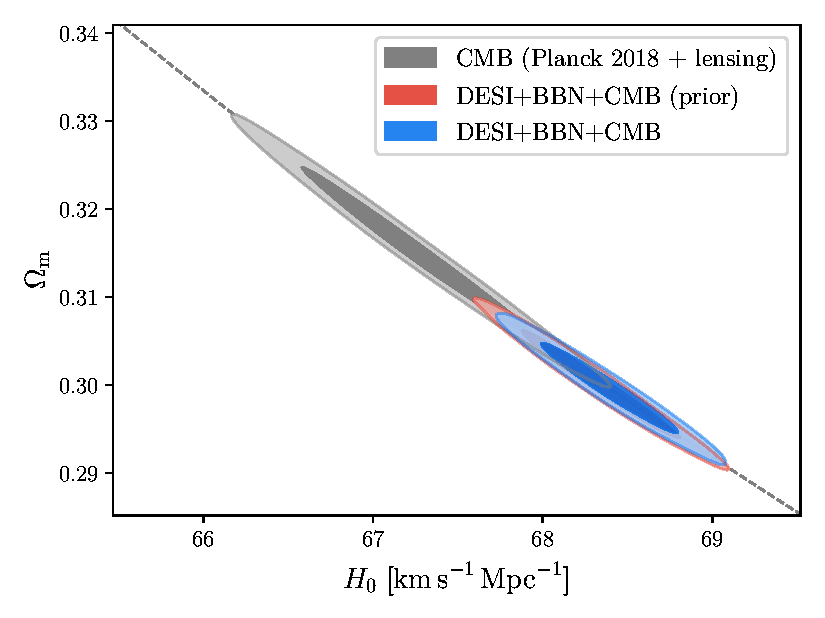
\includegraphics[scale=0.8]{figures/DESI-CMB-H0-omegam.pdf}
\end{figure}

This puts the slight tension between the DESI and CMB datasets and the CMB dataset alone into view. Notice that using the derived CMB prior instead of the full CMB dataset does not affect the posterior distribution all that much. We also note that modifications of \LCDM can alleviate this BAO tension, see \cite{desicollaboration2025desidr2resultsii} for more details.

\subsection*{The Behavior of Dark Energy}

Finally, we discuss some failed attempts to recreate bounds on the behavior of dark energy using the DESI BAO data.
In the base \LCDM model, dark energy is assumed to be constant, i.e. $\rho_\DE(z)/\rho_{\DE,0}=1$. However, it is common to extend the theory by allowing dark energy to have a varying equation of state parameter. The usual parametrization is:
\begin{equation}
w(z)=w_0+w_a(1-a)\quad\implies\quad
  \frac{\rho_\DE(z)}{\rho_{\DE,0}} = a^{3(1+w_0+w_a)}e^{-3w_a(1-a)}.
\end{equation}
This model is known as the \wwCDM model, and can help alleviate some of the tension described earlier in the paper. Note that the ordinary \LCDM model has $w_0=-1$ and $w_a=0$. A non-zero $w_a$ is extremely interesting since it implies that dark energy varies over time. This comes with a host of theoretical problems, and could lead to exciting new physics outside of the \LCDM model.

Perhaps due to a lack of time, some theoretical misunderstanding, or bug in my code, all of my runs involving the \wwCDM model gave me results agreeing with the \LCDM model. I used the DESI DR2 dataset alongside the CMB dataset, including using just the CMB prior to speedup iteration time.

\end{document}
